%instiki:category: FisicaSubatomica
%http://localhost:2500/wiki/show/Cap%C3%ADtulo+II
%% Ilustrar como el teorema de Noether es el mismo
%% para el caso local que global
\chapter{Campos bosónicos}
\label{cha:campos-vectoriales} %noinstiki
%instiki:
%instiki:***
%instiki:
%instiki:[[NotasFS|Tabla de Contenidos]]
%instiki:
%instiki:***
%generated with html2itexTOC instiki_source.html
%instiki:
%instiki:* [Unidades Naturales](#NU)
%instiki:
%instiki:* [Notaci\'on relativista](#srn)
%instiki:
%instiki:  * [Ejemplos de cuadrivectores](#ejemplos_de_cuadrivectores)
%instiki:
%instiki:  * [Ecuaciones covariantes](#ecuac-covar)
%instiki:
%instiki:* [Ecuaciones de Maxwell en notaci\'on covariante](#maxeqs)
%instiki:
%instiki:  * [Lagrangiano Electromagn\'etico](#lagr-electr)
%instiki:
%instiki:  * [Energ\'\i a del campo electromagn\'etico](#energa_del_campo_electromagntico)
%instiki:
%instiki:  * [Fijaci\'on del gauge](#fijacion-del-gauge)
%instiki:
%instiki:* [Ecuaciones de Proca](#ecuacion-de-proca)
%instiki:
%instiki:* [Problemas](#problemas2)
%instiki:
%instiki:***
%instiki:

Hemos visto que la acción para una oscilación mecánica en tres dimensiones se puede escribir en una notación similar a la del producto escalar de un cuadrivector de Lorentz $\partial_\mu\phi$. Cuando dicho campo se interpreta como un campo fundamental, es decir, que su velocidad de propagación es independiente de los sistemas de referencia inerciales, entonces la Acción queda invariante bajo dicho producto escalar.


Se mostrará como la invarianza de la Acción bajo transformaciones de Lorentz es el punto de partida en la construcción de densidades Lagrangianas únicas.

%\subsection{Transformaciones de Lorentz}
%\label{sec:transf-de-lorentz}
\section{Construción de Lagrangianos covariantes}

En está sección vamos a conectar la discusión sobre el Lagrangiano de las vibraciones de la cuerda con las tranformaciones de Lorentz de la relatividad especial. Dicho Lagrangiano tiene hasta ahora la siguiente dependencia funcional $\mathcal{L}(\partial_{\mu}\phi)$.


En la formulación de la teoría clásica de campos debemos asegurarnos de que todos los términos posibles perimtidos por la simetrías asociadas al campo estén presentes en la densidad Lagrangiana. De inmediato surge la pregunta: ¿Qué posibles términos de la forma $\partial_{\mu}\phi$ podrían estar presentes en Lagrangiano?. Antes de responder está pregunta, abordemos el problema algo más general donde la densidad Lagrangiana también depende del campo como mismo
\begin{align*}
  \mathcal{L}(\phi,\partial_\mu \phi)\,.
\end{align*}
En la ecuación~\eqref{eq:dlc3d}, teníamos un Lagragiano en función de $\partial_{\mu}\phi$, y haciendo $v\to c=1$, tenemos
\begin{align}
\label{eq:Lpr}
  \mathcal{L}(\partial_{\mu}\phi)
    =&\frac{1}{2}\left[
      {\partial_0\phi}\,{\partial_0\phi}-\sum_i{\partial_i\phi}\,{\partial_i\phi}
   \right]\nonumber\\
    =&\frac{1}{2}\left[
      {\partial_0\phi}\,{\partial^0\phi}+{\partial_i\phi}\,{\partial^i\phi}
   \right]\nonumber\\
   =&\frac{1}{2}{\partial_\mu\phi}\,{\partial^\mu\phi}\,.
\end{align}
donde se ha usado la convención de suma para índices repetidos. Note que para que la velocidad de propagación sea independiente del sistema de coordenadas se requiere su identificación con la velocidad de la luz. De modo que la queremos interpretar los términos de la densidad Lagrangiana como objetos invariantes, necesariamente se tiene que hacer en el contexto de la relatividad especial.




\section{Transformación de Lorentz para campos escalares}

El campo escalar esta definido por sus propiedades bajo transformaciones de Lorentz. Vamos a estudiar el comportamiento de un campo escalar bajo una transformación general de Lorentz:
\begin{align}
\label{eq:179qft}
  x^\mu\to {x'}^\mu={\Lambda^\mu}_\nu x^\nu\,,
\end{align}
Por definición, el campo escalar no cambia bajo la transformación de Lorentz, es decir, su forma funcional queda inalterada. Por consiguiente el campo escalar debe satisfacer que
\begin{align}
 \phi(x)\to  \phi'(x')=\phi(x)\,,
\end{align}
como se ilustra en la Fig.~\ref{fig:trasla}. La prima en $\phi$ representa el cambio intrínseco en el campo $\phi$ como consecuencia de la transformación. Definimos el cambio correspondiente como
\begin{align}
  \delta \phi(x)=\phi'(x)-\phi(x)\,.
\end{align}


Una transformación de Lorentz infinitesimal,
puede parametrizarse sin perdida de generalidad como
\begin{align}
  x^\mu\to{x'}^\mu=&x^\mu+\delta x^{\mu}\,.
\end{align}

Para visualizar más fácilmente la situación para un campo escalar, supongamos de momento que $\delta x^{\mu}$ corresponde  traslaci\'on espacio--temporal.

Tenemos
\begin{align}
  \phi'(x')&=\phi'(x+\delta x)\\
  &\approx\phi'(x)+\frac{\partial\phi'(x)}{\partial x^\mu}\delta x^\mu\\
  &=[\phi(x)+\delta\phi(x)]+\frac{\partial}{\partial x^\mu}[\phi(x)+\delta\phi(x)]\delta x^\mu\\
  &\approx\phi(x)+\delta\phi(x)+\frac{\partial\phi(x)}{\partial x^\mu}\delta x^\mu,
\end{align}
donde, por simplicidad, $\phi$ es un campo real. Entonces,
\begin{equation}
  \label{eq:Deltaf}
  \Delta\phi(x)\equiv\phi'(x')-\phi(x)=\delta\phi(x)+\frac{\partial\phi(x)}{\partial x^\mu}\delta x^\mu.
\end{equation}
Para una traslaci\'on, $\Delta\phi(x)=0$, ver figura 
\ref{fig:trasla}. %noinstiki([trasla](#fig:trasla)).
De modo que
\begin{equation}
  \label{eq:dmuxmu}
  \delta\phi=-(\partial_\mu\phi)\delta x^\mu,
\end{equation}
y la transformaci\'on del campo $\phi$ como consecuencia de la traslaci\'on es
\begin{align}
  \phi(x)\to\phi'(x)=\phi(x)-\delta\phi(x)=\phi(x)+(\partial_\mu\phi(x))\delta x^\mu\,.
\end{align}
%noinstiki

\begin{figure} %noinstiki
  \centering %noinstiki
  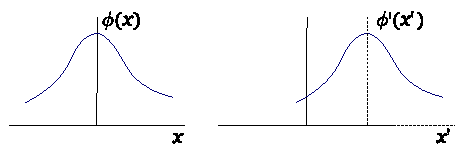
\includegraphics{trasla} %noinstiki
  \caption{Traslaci\'on de funci\'on y coordenadas en una dimensi\'on: $\phi(x)=\phi'(x')$ } %noinstiki
  \label{fig:trasla} %noinstiki
\end{figure} %noinstiki<div id="fig:trasla">Figura trasla:Traslaci\'on de funci\'on y coordenadas $\phi(x)=\phi(x')$ </div>
%noinstiki![trasla](http://gfif.udea.edu.co/figfs/trasla.png)
%noinstiki




Usando la ec.~\eqref{eq:179qft}, tenemos que
\begin{align}
    \phi'(x')=\phi(\Lambda^{-1}x')\,.
\end{align}
Esto es, el campo transformado, evaluado en el punto transformado, da el mismo valor que el campo evaluado en el punto antes de la transformación. 

\begin{frame}[fragile,allowframebreaks]

%Therefore, for an arbitrary space-time point we have that the scalar field transforms under a Lorentz transformation as
Por consiguiente, para un punto del espacio tiempo arbitrario tenemos
que el campo escalar transforma bajo una transformación de Lorentz como
\begin{align}
  \label{eq:scalarlorentz}
 \phi(x)\to  \phi'(x)=\phi(\Lambda^{-1}x)\,.
\end{align}
\end{frame}

Para comprobar la invarianza de Lorentz de la Acción para el campo escalar, necesitamos las propiedades de transformación para $\partial_\mu$. En conveniente invertir la ec.~\eqref{eq:179qft}
\begin{align}
  {\left(\Lambda^{-1}\right)^\mu}_\alpha{x'}^\alpha=&{\left(\Lambda^{-1}\right)^\mu}_\alpha{\Lambda^\alpha}_\nu x^\nu\nonumber\\
=&\delta^\mu_\nu x^\nu\nonumber\\
=&x^\mu\,,
\end{align}
\begin{align}
  \frac{1}{{x'}^\nu}= {\left(\Lambda^{-1}\right)^\mu}_\nu\frac{1}{x^\mu}\,,
\end{align}
o
\begin{align}
  \label{eq:183qft}
    \frac{1}{{x'}^\mu}= {\left(\Lambda^{-1}\right)^\nu}_\mu\frac{1}{x^\nu}\,,
\end{align}
de modo que la transformación de Lorentz para $\partial_\mu=\partial/\partial x^\mu$, es
\begin{align}
  \label{dmulrtran}
   \frac{\partial}{{\partial x'}^\mu}=& {\left(\Lambda^{-1}\right)^\nu}_\mu\frac{\partial}{\partial x^\nu}\nonumber\\
   {\partial\,}'_\mu=& {\left(\Lambda^{-1}\right)^\nu}_\mu\partial_\nu\,,
\end{align}
Podemos ahora demostrar que la Acción obtenida del Lagrangiano en la ec.\eqref{eq:Lpr} es invariante bajo transformaciones de Lorentz haciendo uso de la ec.~(\ref{eq:Lambdacontra}). Para hacer la demostración más general, podemos agregar una función general que solo dependa del campo $\phi$ pero no de sus derivadas, $V(\phi)$
\begin{align}
 \mathcal{L}= \frac{1}{2}{\partial_\mu\phi}\,{\partial^\mu\phi}-V(\phi)\,.
\end{align}
Entonces
\begin{align}
  \mathcal{L}(\phi(x),\partial_{\mu}\phi(x))\to  \mathcal{L}'=& \frac{1}{2}\partial'_\mu\phi'(x)\partial^{'\mu}\phi'(x)-V(\phi'), \nonumber\\
  =&{\left(\Lambda^{-1}\right)^\nu}_\mu g^{\mu \rho}{\left(\Lambda^{-1}\right)^\sigma}_\rho \partial_\nu\phi(\Lambda^{-1}x) \partial_\sigma \phi(\Lambda^{-1}x) -V(\phi')\nonumber\\
  =& g^{\nu \sigma}\partial_\nu\phi(\Lambda^{-1}x) \partial_\sigma \phi(\Lambda^{-1}x) -V(\phi(\Lambda^{-1}x))\nonumber\\
  =& \partial_\nu\phi(\Lambda^{-1}x) \partial^{\nu} \phi(\Lambda^{-1}x) -V(\phi(\Lambda^{-1}x)) \nonumber\\
  =&\mathcal{L}(\phi(\Lambda^{-1}x),\partial_{\mu}\phi(\Lambda^{-1}x))\,.
\end{align}
Ya que la Acción involucra la integración sobre todos los puntos, esta es invariante bajo transformaciones de Lorentz. Explícitamente
\begin{align}
  S\to S'=\int d^4x\, \mathcal{L}
\end{align}

Note que en unidades naturales
\begin{align}
  [S]=[\hbar]=1,
\end{align}
y ya que $[d^4x]=E^{-4}$, entonces
\begin{align}
  [\mathcal{L}]=E^{4}\,.
\end{align}
Como $[\partial_{\mu}]=E$, entonces
\begin{align}
  [\phi]=E\,.
\end{align}

 
Con el cuadrivector \eqref{eq:cv_hatpmu} podemos construir la
siguiente ecuaci\'on
\begin{align}
  \hat{p}_\mu\hat{p}^\mu\phi&=m^2\phi\nonumber\\
  i\partial_\mu i\partial^\mu\phi&=m^2\phi\nonumber\\
  -\partial_\mu\partial^\mu\phi&=m^2\phi\nonumber\\
  \label{eq:waveec}
  \left(\frac{\partial^2}{\partial t^2}-\nabla^2+m^2\right)\phi&=0.
\end{align}
Que corresponde a la ecuaci\'on de Klein-Gordon \eqref{eq:152}. Una expresi\'on escrita en t\'erminos de productos escalares de Lorentz se dice que esta en \emph{forma covariante}. El Lagrangiano covariante que da lugar a
\'esta ecuaci\'on es (ver ec. \eqref{eq:150}
\eqref{eq:15}). %noinstiki[in Cap. I](/wiki/show/Cap%C3%ADtulo+I#eq:15)). 

\begin{equation}
  \label{eq:wavelagtrue}
  \mathcal{L}=\frac{1}{2}\partial_\mu\phi\partial^\mu\phi-\frac{1}{2}m^2\phi^2
\end{equation}
El Lagrangiano m\'as general posible para el campo $\phi$ es en general bastante arbitrario:
\begin{equation}
  \mathcal{L}=\frac{1}{2}\partial_\mu\phi\partial^\mu\phi-V(\phi)\,,
\end{equation}
donde $V(\phi)$ es una función de campos escalar real $\phi$. Si $V(\phi)$ es una función polinómica del campo $\phi$, tenemos por ejemplo.
\begin{equation}
  \label{eq:wavelag}
  \mathcal{L}=\frac{1}{2}\partial_\mu\phi\partial^\mu\phi-\frac{1}{2}m^2\phi^2+\frac{1}{4}\lambda\phi^4+a\phi+b\phi^3.
\end{equation}
Un t\'ermino de la forma $\partial_\mu\partial^\mu\phi$ puede reabsorverse en la
ec.~\eqref{eq:wavelag} como una derivada total. Un posible t\'ermino
$J_\mu\partial^\mu\phi$, con $J_\mu$ constante, tambi\'en puede reescribirse como una
derivada total. Un t\'ermino constante
no afecta las ecuaciones de movimiento. Imponer la simetr\'\i a $\phi\to-\phi$
anula los dos \'ultimos t\'erminos. Potencias de $\phi$ mayores de cuatro
dar\'\i a lugar a una Teor\'\i a Cu\'antica de Campos no renormalizable. 

La dimensi\'on del campo $\phi$ puede obtenerse usando que la acci\'on es adimensional
\begin{equation}
  [S]\supset\left[\int d^4x\,m^2\phi^2\right]=E^{-4}E^2[\phi]^2\to [\phi]=E^1
\end{equation}
Diremos entonces que la dimensi\'on de $\phi$ es 1 (en unidades de energ\'\i a). Similarmente
\begin{equation}
  [S]\supset\left[\int d^4x\,\partial_\mu\phi\partial^\mu\phi\right]=E^{-4}[\partial_\mu]^2E^2\to [\partial_\mu]=E^1
\end{equation}
Como era de esperarse debido a que la derivada tiene unidades de longitud inversa.

Si hacemos $\lambda=a=b=0$ en la ec.~\eqref{eq:wavelag}, y usando las
ecuaciones de Euler-Lagrange \eqref{eq:eelcallfmu}, se obtiene
\begin{align}
  (\hat{p}_\mu\hat{p}^\mu-m^2)\phi&=0\nonumber\\
  \label{eq:k-gpmu} %noinstiki
(\hat{E}^2-\hat{\mathbf{P}}^2-m^2)\phi&=0\\
\label{eq:kg} 
  (\Box+m^2)\phi&=0,
\end{align}
donde
\begin{equation}
  \label{eq:dalambertiano}
  \Box\equiv\partial_\mu\partial^\mu=\frac{\partial^2}{\partial t^2}-\nabla^2. 
\end{equation}
Es el D'Alembartiano~\cite{daelembertiano}. 
Ec.~\eqref{eq:k-gpmu} %noinstikiEc.~\eqref{eq:kg}
corresponde a la forma de operadores de la
ecuaci\'on de energ\'\i a-momentum relativista. La
ec.~\eqref{eq:kg} se conoce como la ecuaci\'on de Klein-Gordon, con
Lagrangiano
\begin{equation}
  \label{eq:kglag}
  \mathcal{L}=\frac{1}{2}\partial_\mu\phi\partial^\mu\phi-\frac{1}{2}m^2\phi^2, 
\end{equation}
Una expresi\'on escrita en t\'erminos de productos escalares de
Lorentz se dice que esta en \emph{forma covariante}. Por lo tanto la
ecuaci\'on de Klein--Gordon y su correspondiente Lagrangiano est\'an
en forma covariante. Tambi\'en tienen la simetr\'\i a
$\phi\to-\phi$. A $\phi$ se le denomina \emph{campo escalar}.


%\begin{frame}[fragile,allowframebreaks]
% The field $A^\mu(x)$ transforms simultaneously as field and as vector under Lorentz transformation
% \begin{align}
%   A^\mu(x)\to {A'}^\mu(x')={\Lambda^\mu}_\nu A^\nu(\Lambda^{-1}x)\,.
% \end{align}
%\end{frame}

 
\section{Principio de mínima acción para campos}
%También hemos visto que adicionar una función del campo $V(\phi)$, la invarianza de la acción se mantiene.

Establecemos el \emph{principio de mínima acción para campos} de la siguiente manera: La acción más general posible para un conjunto de campos contiene todos los posibles productos escalares entre los campos y sus derivadas, con las siguientes restricciones
\begin{enumerate}
\item La dimensión de los campos y derivadas en cada término de la correspondiente densidad lagrangiana debe ser menor o igual a cuatro.
\item La densidad Lagrangiana no debe contener derivadas altas (máximo dos derivadas)
\item Los campos fundamentales se deben anular a espacio infinito.
\end{enumerate}




Con estas restricciones es suficiente mantener los primeros cuatro términos de la expansión de Taylor de $V(\phi)$ (el término constante se puede remover redefiniendo el estado de mínima energía)
\begin{align}
  V(\phi)=a \phi + b\phi^2+c\phi^4+d\phi^4\,,
\end{align}

La última condición excluye términos del tipo
\begin{align}
  \partial_\mu \partial^\mu \phi\,,   \phi\partial_\mu \partial^\mu \phi\,.
\end{align}
De modo que la densidad Lagrangiana más general posible para un campo escalar real es
\begin{align}
  \frac{1}{2}{\partial_\mu\phi}\,{\partial^\mu\phi}+a \phi + b\phi^2+c\phi^4+d\phi^4\,.
\end{align}

Realizaciones propuestas para este campo escalar incluye el de un campo de materia oscura con un potencial tipo oscilador armónico.
% figura
Pero una realización ya encontrada en la naturaleza corresponde al campo de Higgs con un potencial tipo ruptura expontánea de vacio

Una realización física para la acción del campo escalar real con un potencia escalar tipo ``slow-roll''  corresponde al campo del inflatón en cosmología.

\section{Campo escalar complejo}
Entre más simetrías posea una Acción menos arbitraría es. Podemos
ilustrar esta afirmación si consideramos una Acción para un campo escalar
complejo que además de ser invariante de Lorentz, es además invariante
bajo transformaciónes de fase.


Para un campo complejo con invarianza de fase, el potencial $V(\phi,\phi^{*})$ es único:
\begin{align}
\label{eq:cef}
  \mathcal{L}=\partial_{\mu}\phi^{*} \partial^{\mu}\phi-m^2\phi^{*}\phi+\lambda \left(\phi^{*}\phi \right)^2\,.
\end{align}
En efecto, la densidad Lagrangiana y por consiguiente la Acción, son invariante bajo la transformación
\begin{align}
  \phi\to \phi'=\operatorname{e}^{i\theta}\phi\,,\qquad \text{$\theta$ constante}\,.
\end{align}
Para $\theta$ infinitesimal
\begin{align}
\label{eq:deltaphi}
  \delta\phi=\phi'-\phi=i\theta\phi
\end{align}



Por lo tanto
\begin{align}
  \left[ m \right]=&E& \left[ \lambda \right]=&1\,.
\end{align}


Términos de orden superior se pueden obtener a partir de esa
Lagrangiana única y por eso no se consideran. 
No se consideran términos con derivadas superiores porque al igual que en mecánica clásica pueden generar inestabilidades. Por lo tanto, los únicos términos con derivadas que dejen invariante la acción bajo transformaciones de Lorentz son (el primero sólo es posible para un campo real):
\begin{align}
  \partial_{\mu}\partial^{\mu}\phi,\qquad \phi^{*}\partial_{\mu}\partial^{\mu}\phi\,.
\end{align}
Una densidad Lagrangiana incluyendo estos términos se puede reescribir en términos de la densidad Lagranginan en la ec.~\eqref{eq:cef}, hasta una deriva total. Por ejemplo
\begin{align}
  \mathcal{L}_{\text{new}}=&-\phi^{*}\partial_{\mu}\partial^{\mu}\phi-m^2\phi^{*}\phi+\lambda \left(\phi^{*}\phi \right)^2\,\nonumber\\
=&\partial_{\mu}\phi^{*}\partial^{\mu}\phi\,-\partial_{\mu}\left(\phi^{*}\partial^{\mu}\phi\right)-m^2\phi^{*}\phi+\lambda \left(\phi^{*}\phi \right)^2\,\nonumber\\
=&\mathcal{L}-\partial_{\mu}\left(\phi^{*}\partial^{\mu}\phi\right)\,.
\end{align}
En general, si comparamos dos acciones que difieran en la derivada total de algún $X^{\mu}$ (en el caso anterior $X^{\mu}=-\phi^{*}\partial^{\mu}\phi$)
\begin{align}
  S_{\text{new}}=S+\int \partial_{\mu}\left(\phi^{*}\partial^{\mu}\phi\right)d^4x\,.
\end{align}
Veremos más adelante que la integral de una derivada total, con las condiciones de frontera adecuadas, no contribuye a la Acción.

\begin{frame}[fragile,allowframebreaks]


En ese caso la Acción, y la correspondiente densidad Lagrangiana son
únicas y están dadas por una función polinómica de $\phi^{*}\phi$
\begin{align}
  \mathcal{L}=\partial_{\mu}\phi^{*} \partial^{\mu}\phi-m^2\phi^{*}\phi+\lambda \left(\phi^{*}\phi \right)^2\,.
\end{align}
\end{frame}

De las ecuaciones de Euler-Lagrange para $\phi^*$, usando el Lagrangiano en ec.~(\ref{eq:41qft})
\begin{align}
  \partial_\mu\left[
      \frac{\partial\mathcal{L}}{\partial(\partial_\mu\phi^*)}\right]-\frac{\partial\mathcal{L}}{\partial\phi^*}&=0\nonumber\\
    \partial_\mu\partial^\mu\phi+m^2\phi&=0\nonumber\\
    \label{eq:43qft}
    (\Box+m^2)\phi&=0,
\end{align}
y de la ecuaciones de Euler-Lagrange para $\phi$,
\begin{equation}
  \label{eq:44qft}
    (\Box+m^2)\phi^*=0.
\end{equation}
De este modo tanto $\phi$, como $\phi^*$, satisfacen la ecuación de Klein-Gordon. Cada campo además corresponde a una partícula de masa $m$ como en el caso de $\phi_1$ y $\phi_2$

Estamos ahora interesado en las simetrías internas del Lagrangiano. Entonces la corriente conservada puede definida en la sección~\ref{sec:principio-de-minima-call}, eq.~\eqref{eq:jmuphi}
\begin{align}
  J^\mu=&\frac{\partial\mathcal{L}}{\partial(\partial_\mu\phi)}\delta\phi+\delta\phi^*\frac{\partial\mathcal{L}}{\partial(\partial_\mu\phi^*)}\nonumber\\
  \label{eq:45qft}
  J^\mu=&\partial^\mu\phi^*\delta\phi+\delta\phi^*\partial^\mu\phi.
\end{align}
Además de la invarianza de Lorentz, el Lagrangiano en ec,~(\ref{eq:41qft}) también es invariante bajo el grupo de transformaciones U(1) definido en las sección~\ref{sec:lagr-electr}, pero con una fase constante
\begin{equation*}
  U=e^{i\theta}\approx1+i\theta.
\end{equation*}
Entonces
\begin{align}
  \phi\overset{U}{\longrightarrow}\phi'&=e^{i\theta}\phi\approx(1+i\theta)\phi\nonumber\\
  &=\phi+i\theta\phi.
\end{align}
Entonces,
\begin{align}
  \delta\phi&=i\theta\phi\\
  \delta\phi^*&=-i\theta\phi^*.
\end{align}
Reemplazando en ec.~(\ref{eq:45qft})
\begin{equation}
\label{eq:46qft}
  J^\mu\propto -i\theta(\phi\partial^\mu\phi^*-\phi^*\partial^\mu\phi),
\end{equation}
y
\begin{equation}
\label{eq:47qft}
  \rho=J^0\propto-i\theta(\phi\frac{\partial\phi^*}{\partial t}-\phi^*\frac{\partial\phi}{\partial t}).
\end{equation}
Definimos $J^\mu$ como
\begin{equation}
  \label{eq:48qft}
   J^\mu= i(\phi^*\partial^\mu\phi-\phi\partial^\mu\phi^*),
\end{equation}
Como $\rho$ puede ser negativo no puede interpretarse como una
probalidad, como se hizo con la función de onda de la ecuación de
Scrödinger. Esto presentó un obstaculo en la interpretación inicial de
la ecuación de Klein-Gordon. Sin embargo una vez se cuantiza el
campo escalar la probabilidad de los estados cuánticos queda bien
definida \cite{Gross}. 

\section{Invarianza de fase local para campo escalar complejo}

Aplicando el principio gauge local al Lagrangiano para un campo escalar complejo presentado en la ecuación~\ref{eq:cef} con $\lambda=0$, debemos reemplazar la derivada normal $\partial_{\mu}$, por la derivada covariante $\mathcal{D}_{\mu}=\partial_{\mu}+iq A_{\mu}$ y adicionar todos los términos invariantes asociados al campo $A_\mu$, de modo que
\begin{align}
\label{eq:lcv}
  \mathcal{L}=& \left( \mathcal{D}_{\mu} \phi \right)^{*} \mathcal{D}^{\mu}\phi -m^2 \phi^{*}\phi-\frac{1}{4}F^{\mu\nu}F_{\mu\nu} \nonumber\\
             =&\left( \partial_{\mu}\phi^{*}-iq A_{\mu} \phi^{*} \right)\left( \partial^{\mu}\phi+iq A^{\mu} \phi \right) -m^2 \phi^{*}\phi-\frac{1}{4}F^{\mu\nu}F_{\mu\nu} \nonumber\\
              =&\partial_{\mu}\phi^{*}\partial^{\mu}\phi-m^2 \phi^{*}\phi+iq \left(\phi\partial_{\mu}\phi^{*} -\phi^{*}\partial_{\mu}\phi \right) A^{\mu} +q^2 \phi^{*}\phi A_{\mu} A^{\mu} -\frac{1}{4}F^{\mu\nu}F_{\mu\nu} 
\end{align}
De modo que
\begin{align}
  \partial_{\mu} \left[ \frac{\partial \mathcal{L}}{\partial \left( \partial_{\mu}\phi^{*} \right)} \right]-\frac{\partial \mathcal{L}}{\partial \phi^{*}}
=&\partial_{\mu} \left( \partial^{\mu}+iq A^{\mu} \right)\phi -\left(-iq \partial_{\mu}\phi A^{\mu} +q^2 A_{\mu}A^{\mu}\phi-m^{2}\phi  \right) \nonumber\\
 =&\partial_{\mu} \left( \partial^{\mu}+iq A^{\mu} \right)\phi  +iq \partial_{\mu}\phi A^{\mu}-q^2 A_{\mu}A^{\mu}\phi+m^{2}\phi\,.
\end{align}

Por lo tanto
\begin{align}
-iq &\phi^{*} \left\{\partial_{\mu} \left[ \frac{\partial \mathcal{L}}{\partial \left( \partial_{\mu}\phi^{*} \right)} \right]-\frac{\partial \mathcal{L}}{\partial \phi^{*}} \right\}   
= -iq \phi^{*}\partial_{\mu}\left( \partial^{\mu}+iq A^{\mu} \right)\phi+q^2 A_{\mu}  \phi^{*} \partial^{\mu}\phi +iq^3 A_{\mu}A^{\mu}\phi^{*}\phi-iq m^2\phi^{*}\phi \nonumber\\
  =& -iq \partial_{\mu} \left[ \phi^{*}\left( \partial^{\mu}+iq A^{\mu} \right)\phi \right]+iq \left( \partial_{\mu} \phi^{*}\right)\left( \partial^{\mu}+iq A^{\mu} \right)\phi +q^2 A_{\mu}  \phi^{*} \partial^{\mu}\phi +iq^3 A_{\mu}A^{\mu}\phi^{*}\phi-iq m^2\phi^{*}\phi \nonumber\\
  =& -iq \partial_{\mu} \left[ \phi^{*}\mathcal{D}^{\mu}\phi \right]+iq  \partial_{\mu} \phi^{*}\partial^{\mu}\phi-q^2A^\mu \left( \partial_{\mu} \phi^{*} \right)\phi  +q^2 A_{\mu}  \phi^{*} \partial^{\mu}\phi +iq^3 A_{\mu}A^{\mu}\phi^{*}\phi-iq m^2\phi^{*}\phi\,. 
\end{align}
Similarmente
\begin{align}
  iq &\left\{\partial_{\mu} \left[ \frac{\partial \mathcal{L}}{\partial \left( \partial_{\mu}\phi \right)} \right]-\frac{\partial \mathcal{L}}{\partial \phi} \right\} \phi \nonumber\\
  =& iq \partial_{\mu} \left[ \left(  \mathcal{D}^{\mu}\phi \right) \phi^{*} \right]-iq  \partial_{\mu} \phi^{*}\partial^{\mu}\phi+q^2A^\mu \left( \partial_{\mu} \phi^{*} \right)\phi  -q^2 A_{\mu}  \phi^{*} \partial^{\mu}\phi -iq^3 A_{\mu}A^{\mu}\phi^{*}\phi+iq m^2\phi^{*}\phi\,. 
\end{align}
Sumando las dos expresiones, todos los términos con excepción de los primeros se cancelan entre si, dando lugar a 
\begin{align}
   \sum_{i}\mathcal{E}_{i} a_{\alpha i}=& \partial_{\mu} j^{\mu}\,,
\end{align}
donde
\begin{align}
  j^{\mu}=-iq \left[  \phi^{*}\mathcal{D}^{\mu}\phi -  \left(  \mathcal{D}^{\mu}\phi \right)^{*} \phi\right]\,,
\end{align}
que corresponde a la carga eléctrica. Note que dicho resultado se puede obtener más directamente usando la ec.~\eqref{eq:tnoeth2}.

Note además que 
\begin{align}
\mathcal{D}_{\mu}\mathcal{D}^{\mu}\phi=  \left( \partial_{\mu}+iq A_{\mu}  \right)\left( \partial^{\mu}+iq A^{\mu} \right)\phi=& \partial_{\mu}\left( \partial^{\mu}+iq A^{\mu} \right)\phi+iq A_{\mu}  \left( \partial^{\mu}+iq A^{\mu} \right)\phi \nonumber\\
=& \partial_{\mu}\left( \partial^{\mu}+iq A^{\mu} \right)\phi+iq A_{\mu}   \partial^{\mu}\phi -q^2 A_{\mu}A^{\mu}\phi\,.
\end{align}
Por lo tanto la ecuación de movimiento asociada al campo $\phi^{*}$



\begin{align}
  \partial_{\mu} \left[ \frac{\partial \mathcal{L}}{\partial \left( \partial_{\mu}\phi^{*} \right)} \right]-\frac{\partial \mathcal{L}}{\partial \phi}=&
 \left(\mathcal{D}_{\mu}\mathcal{D}^{\mu}+m^2  \right)\phi\,=0
\end{align}
Que corresponde a la ecuación de Klein-Gordon pero con la derivada normal reemplazada por la derivada covariante.

Partiendo de nuevo de \ref{eq:lcv}, es interesenta notar que



\section{Ecuaciones de Maxwell en notaci\'on covariante }
\label{sec:maxeqs}

\begin{align*}
  \mathcal{L}(A_0,\partial_\mu A_0)=  \mathcal{L}(\phi,\partial_\mu \phi)\,.
\end{align*}


Ecuaciones homog\'eneas:
\begin{align}
  \label{eq:hom_m_eq}
  \boldsymbol{\nabla}\cdot\mathbf{B}&=0,&\boldsymbol{\nabla}\times\mathbf{E}+\frac{\partial\mathbf{B}}{\partial t}&=0
\end{align}
Ecuaciones inhomog\'eneas:
\begin{align}
  \label{eq:inhom_m_eq}
  \boldsymbol{\nabla}\cdot\mathbf{E}&=\rho,&\boldsymbol{\nabla}\times\mathbf{B}-\frac{\partial\mathbf{E}}{\partial t}&=\mathbf{J}.
\end{align}
La primera ecuaci\'on establece la ausencia de cargas magn\'eticas, la segunda corresponde a la Ley de Faraday y la tercera a la Ley de Gauss. La cuarta sin el t\'ermino de desplazamiento el\'ectrico introducido por Maxwell corresponde a la Ley de Amp\`ere
\begin{equation}
   \boldsymbol{\nabla}\times\mathbf{B}=\mathbf{J}.
\end{equation}
Tomando la divergencia en esta expresi\'on tenemos
\begin{equation}
  \boldsymbol{\nabla}\cdot\mathbf{J}=0,
\end{equation}
que corresponde a la ecuaci\'on de continuidad \eqref{eq:conti} para $\rho$ constante
\begin{equation}
  \label{eq:153}
  \frac{\partial \rho}{\partial t}+\boldsymbol{\nabla}\cdot\mathbf{J}=0.
\end{equation}
De este modo la Ley de Amp\`ere da lugar a la conservaci\'on de carga el\'ectrica pero solo a nivel global:  una perdida de carga el\'ectrica en un punto del universo puede ser compensada por la aparici\'on instant\'anea de carga el\'ectrica en otro lugar del universo. La conservaci\'on global podr\'\i a necesitar la propagaci\'on instant\'anea de se\~nales, y esto est\'a en conflicto con la relatividad especial.


Tomando la divergencia de la Ley de Amp\`ere modificada por Maxwell
\begin{equation}
   \boldsymbol{\nabla}\times\mathbf{B}-\frac{\partial\mathbf{E}}{\partial t}=\mathbf{J},
\end{equation}
obtenemos la ecuaci\'on de continuidad \eqref{eq:153}. Dicha ecuaci\'on establece que la raz\'on de decrecimiento de la carga en un volumen arbitrario $V$ es debido precisa y \'unicamente al flujo de la corriente fuera de su superficie; de modo que la carga no puede ser creada ni destruida dentro de $V$.  Ya que $V$ puede ser arbitrariamente peque\~no esto significa que la carga el\'ectrica debe conservarse localmente.   El t\'ermino extra introducido por Maxwell est\'a motivado por un requerimiento de conservaci\'on local. 

A la luz del teorema de Noether la conservaci\'on local de la carga el\'ectrica debe provenir de una transformaci\'on continua y \emph{local} que deje invariante a la ecuaciones de Maxwell. Las invarianza gauge de la ecuaciones de Maxwell juegan este papel. Las cargas conservadas localmente pueden determinarse a partir de la din\'amica del sistema  \cite{Aitchison:2003tq}, adem\'as del uso de cargas conocidas que participen en alguna reacci\'on. Por ejemplo se puede estudiar la forma como responde una part\'\i cula de carga desconocida a campos electromagn\'eticos para determinar su carga. 

El principio gauge local, que pretendemos formular, va m\'as all\'a del teorema de Noether estableciendo una relaci\'on entre las simetr\'\i as, las leyes de conservaci\'on y la din\'amica. Este se constituye en el paradigma para estudiar las interacciones relevantes en f\'\i sica de part\'\i culas.

Para mostrar la invarianza gauge que exhiben las ecuaciones de Maxwell, es conveniente reescribirlas en forma covariante. Para ello es conveniente usar el potencial escalar el\'ectrico $\phi$ y el potencia vectorial magn\'etico $\mathbf{A}$.

%to_en:The following equations are equivalent to the two homogenous Maxwell equations
Las siguientes ecuaciones son equivalentes a las ecuaciones homog\'eneas de Maxwell
\begin{align}
  \label{eq:phia}
  \mathbf{E}&=-\boldsymbol{\nabla}\phi-\frac{\partial\mathbf{A}}{\partial t}&
  \mathbf{B}&=\boldsymbol{\nabla}\times\mathbf{A}.
\end{align}
Ya que
\begin{align*}
  \boldsymbol{\nabla}\times\mathbf{E}&=-\boldsymbol{\nabla}\times\boldsymbol{\nabla}\phi-\frac{\partial}{\partial t}\boldsymbol{\nabla}\times\mathbf{A}\\
  &=-\frac{\partial\mathbf{B}}{\partial t},
\end{align*}
y
\begin{align*}
  \boldsymbol{\nabla}\cdot\mathbf{B}&=\boldsymbol{\nabla}\cdot(\boldsymbol{\nabla}\times\mathbf{A})\\
  &=0
\end{align*}
Usando el cuadrivector en ec.~(\ref{eq:cv_phia}) y
expandiendo la ec.~(\ref{eq:phia}), tenemos
\begin{align}
  E^i&=-(\frac{\partial A^0}{\partial x^{i}}+\frac{\partial A^{i}}{\partial x^0})\nonumber\\
  &=(\frac{\partial A^0}{\partial x_i}-\frac{\partial A^{i}}{\partial x_0})\nonumber\\
  &=\partial^{i}A^0-\partial^0 A^{i}\nonumber\\
  \label{eq:Efmunu}
  &=\partial^\mu A^\nu-\partial^\nu A^\mu,
  \qquad 
  \mu=i,\quad \nu=0\\
  \label{eq:E_Fi0} %noinstiki
  E^{i}&=F^{i0}
\end{align}
donde hemos definido el Tensor de intensidad electrom\'agnetica como:
\begin{equation}
  \label{eq:fmunu}
    F^{\mu\nu}=\partial^\mu A^\nu-\partial^\nu A^\mu.
\end{equation}
A $A^\mu$ se le denomina \emph{campo vectorial}. Similarmente
\begin{align}
  B^k&=\epsilon_{ijk}\frac{\partial A^j}{\partial x^{i}}\nonumber\\
  \epsilon_{lmk}B^k&=\epsilon_{lmk}\epsilon_{ijk}\frac{\partial A^j}{\partial x^{i}}\nonumber\\
  &=(\delta_{li}\delta_{mj}-\delta_{lj}\delta_{mi})\frac{\partial A^j}{\partial x^{i}}\nonumber\\
  &=\frac{\partial A^m}{\partial x^l}-\frac{\partial A^l}{\partial x^m}\nonumber\\
  &=-\frac{\partial A^m}{\partial x_l}+\frac{\partial A^l}{\partial x_m}\nonumber\\
  &=\partial^m A^l-\partial^l A^m\nonumber\\
  \label{eq:Bfmunu}
  &=\partial^\mu A^\nu-\partial^\nu A^\mu,
  \qquad 
  \mu=m,\quad \nu=l.\\
  \label{eq:BFij}
\epsilon_{lmk}B^k&=F^{ml}
\end{align}
Por consiguiente la ec.~(\ref{eq:fmunu}) es tambi\'en equivalente a las
dos ecuaciones homog\'eneas de Maxwell. En forma matricial,
\begin{align}
  F^{\mu\nu}&=
  \begin{pmatrix}
    0       &\partial^0A^1-\partial^1A^0&\partial^0A^2-\partial^2A^0&\partial^0A^3-\partial^3A^0\\
    \partial^1A^0-\partial^0A^1&0       &\partial^1A^2-\partial^2A^1&\partial^1A^3-\partial^3A^1\\
    \partial^2A^0-\partial^0A^2&\partial^2A^1-\partial^1A^2&0       &\partial^2A^3-\partial^3A^2\\
    \partial^3A^0-\partial^0A^3&\partial^3A^1-\partial^1A^3&\partial^3A^2-\partial^2A^3&0\\
  \end{pmatrix}\nonumber\\
  &=
  \begin{pmatrix}
    0 &-E^1   &-E^2   &-E^3   \\    
    E^1&0     &\epsilon_{213}B^3&\epsilon_{312}B^2\\
    E^2&\epsilon_{123}B^3&0     &\epsilon_{321}B^1\\
    E^3&\epsilon_{132}B^2&\epsilon_{231}B^1&0\\
  \end{pmatrix}\nonumber\\
  &=
\label{eq:matrixfmunu}
  \begin{pmatrix}
    0 &-E^1&-E^2&-E^3   \\    
    E^1&0  &-B^3&B^2\\
    E^2&B^3 &0  &-B^1\\
    E^3&-B^2&B^1 &0\\
  \end{pmatrix}.
\end{align}

La ec.~(\ref{eq:fmunu}) satisface la identidad,
\begin{equation}
  \label{eq:homME3}
  \partial^\lambda F^{\mu\nu}+\partial^\mu F^{\nu\lambda}+\partial^\nu F^{\lambda\mu}=0
\end{equation}
Definiendo el tensor dual como
\begin{equation*}
  \tilde{F}^{\mu\nu}=\frac{1}{2}\epsilon^{\mu\nu\rho\sigma}F_{\rho\sigma},
\end{equation*}
la ec.~(\ref{eq:homME3}) puede escribirse como
\begin{equation}
  \label{eq:homEM4}
  \partial_\mu\tilde{F}^{\mu\nu}=0.
\end{equation}

Para reescribir las ecuaciones de Maxwell inhomog\'enas en forma
covariante usaremos adem\'as el cuadrivector $J^\mu$ de la
ec.~\eqref{eq:cv_jmu}.  Usando la ec.~\eqref{eq:Efmunu}, la primera
ecuaci\'on de Maxwell inhomog\'enea~\eqref{eq:inhom_m_eq} puede escribirse
como
\begin{align}
  \label{nohomME21}
    \frac{\partial E^{i}}{\partial x^{i}}&=J^0\nonumber\\
    \frac{\partial}{\partial x^{i}}F^{i0}&=J^0\nonumber\\
    \partial_iF^{i0}&=J^0\nonumber\\
    \partial_\mu F^{\mu0}&=J^0\,.
\end{align}
Usando las ecs.~\eqref{eq:Efmunu}, \eqref{eq:Bfmunu}, la segunda
ecuaci\'on de Maxwell inhomog\'enea~\eqref{eq:inhom_m_eq} puede escribirse
como
\begin{align}
  \epsilon_{ijk}\frac{\partial B^j}{\partial x^{i}}-\frac{\partial E^k}{\partial t}&=J^k\nonumber\\
  -\frac{\partial (\epsilon_{ikj}B^j)}{\partial x^{i}}-\frac{\partial E^k}{\partial t}&=J^k\nonumber\\
-\partial_iF^{ki}-\partial_0F^{k0}&=J^k\nonumber\\
\partial_iF^{ik}+\partial_0F^{0k}&=J^k\nonumber\\
\label{nohomME22}
\partial_\mu F^{\mu k}&=J^k
\end{align}

Las ecuaciones \eqref{nohomME21},
\eqref{nohomME22} pueden escribirse en forma compacta como
\begin{align}
\label{eq:nohomME2}
  \partial_\mu F^{\mu\nu}&=J^\nu\\
&=
\begin{cases}
  \partial_\mu(\partial^\mu A^0-\partial^0A^{i})=J^0&\text{para $\nu=0$}\\
  \partial_\mu(\partial^\mu A^{i}-\partial^{i}A^\mu)=J^{i}&\text{para $\nu=i$}
\end{cases}\nonumber
\end{align}


Los resultados sobre la notaci\'on covariante de la ecuaciones de Maxwell est\'an resumidos en la Tabla~\ref{tab:eqmax} %noinstiki
\begin{table} %noinstiki
  \begin{center} %noinstiki
  \begin{tabular}{l|l|l|l} %noinstiki
            &$\mathbf{E}$, $\mathbf{B}$&$A^\mu$            &$F^{\mu\nu}$\\\hline %noinstiki
Homog\'eneas  &Ec.~(\ref{eq:hom_m_eq})   &~(\ref{eq:phia})&~(\ref{eq:fmunu}) \'o (\ref{eq:homME3}) \'o (\ref{eq:homEM4})\\\hline %noinstiki
Inhomog\'eneas& (\ref{eq:inhom_m_eq})    &                &~\eqref{eq:nohomME2} \\ %noinstiki
  \end{tabular} %noinstiki
  \end{center} %noinstiki
  \caption{Ecuaciones de Maxwell} %noinstiki
  \label{tab:eqmax} %noinstiki
\end{table} %noinstiki
De la parte izquierda de la ecuaci\'on \eqref{eq:nohomME2}, podemos ver que
\begin{align*}
  \partial_\nu\partial_\mu F^{\mu\nu}&=0
\end{align*}
Por consiguiente, la cuadricorriente $J^\mu$ es conservada:
\begin{equation}
  \label{eq:consvjmu}
  \partial_\mu J^\mu=0
\end{equation}


\subsection{Lagrangiano Electromagn\'etico}
\label{sec:lagr-electr}
%to_en:Eq.~(\ref{eq:phia}) is invariant under the following transformations
La ec.~(\ref{eq:phia}) es invariante bajo las siguientes transformaciones
\begin{align}
  \label{eq:phia_transf}
  \mathbf{A}&\to\mathbf{A}'=\mathbf{A}+\boldsymbol{\nabla}\chi&
  \phi&\to\phi'=\phi-\frac{\partial\chi}{\partial t} 
\end{align}
%to_en:Since
Ya que
\begin{equation}
  \label{eq:Etrans}
  \mathbf{E}\to\mathbf{E}'= -\boldsymbol{\nabla}\phi+\frac{\partial}{\partial t}\boldsymbol{\nabla}\chi
  -\frac{\partial\mathbf{A}}{\partial t}-\frac{\partial}{\partial t}\boldsymbol{\nabla}\chi=\mathbf{E}
\end{equation}
\begin{equation}
  \label{eq:btransf}
  \mathbf{B}\to\mathbf{B}'= \boldsymbol{\nabla}\times\mathbf{A}+
  \underbrace{\boldsymbol{\nabla}\times\boldsymbol{\nabla}\chi}_{\displaystyle =0}=\mathbf{B}
\end{equation}
%to_en:This imply that different observers in different space points, using different calibrations for their measures, get the same fields. 
Esto implica que diferentes observadores en diferentes puntos del espacio, usando diferentes calibraciones para sus medidas, obtienen los mismos campos. Las  ecs.~\eqref{eq:phia_transf}, corresponden a \emph{transformaciones gauge locales}

%to_en:In covariant notation
En notaci\'on de cuadrivectores
\begin{align}
  A^\mu\to {A'}^\mu=&\left(\phi-\frac{\partial\chi}{\partial t},\mathbf{A}+\boldsymbol{\nabla}\chi
  \right)\nonumber\\
  =&\left(\phi-\frac{\partial\chi}{\partial t},A^{i}+\partial_i\chi
  \right)\nonumber\\
  =&\left(\phi-\partial^0\chi,A^{i}-\partial^{i}\chi
  \right)\nonumber\\
  =&\left(\phi,A^{i}
  \right)-
  \left(
    \partial^0\chi,\partial^{i}\chi
  \right)\nonumber\\
  \label{eq:aphicov}
  A^\mu\to {A'}^\mu=&A^\mu-\partial^\mu\chi
\end{align}
%to_en: Let $U$ an element of the Transformation Group $U(1)$:
Sea  $U$ un elemento del Grupo de Transformaciones  $U(1)$:
\begin{equation}
  \label{eq:u1ele}
  U=e^{i\theta(x)}\in U(1)
\end{equation}
%to_en: The Group is defined by the infinity set of elements $U_i=e^{i\theta(x_i)}$. Then
El Grupo est\'a definido por el conjunto infinito de elementos $U_i=e^{i\theta(x_i)}$. Entonces
\begin{itemize} %noinstiki
%instiki:
\item Producto de Grupo 
  \begin{equation*}
      U_1\cdot U_2=e^{i[\theta(x_1)+\theta(x_2)]}\equiv e^{i\theta(x_3)}\in U(1)
  \end{equation*}
\item Identidad: 
  \begin{equation*}
  \theta(x)=0\qquad \text{tal que}\qquad U_I=1  
  \end{equation*}
\item Inverso 
  \begin{equation*}
      \theta(-x)=-\theta(x)\qquad \text{tal que}\qquad U^{-1}=e^{-i\theta(x)}
  \end{equation*}
\end{itemize} %noinstiki
Note que si
\begin{equation}
  \label{eq:amutransf}
  A^\mu\to{A'}^\mu=A^\mu-\frac{i}{e}(\partial^\mu U)U^{-1}
\end{equation}
%to_en:(If $\theta(x)=$cte, $ A^\mu={A^\mu}'$, phase invariance). If $\theta$ is sufficiently small
(Si $\theta=$cte, $ A^\mu={A'}^\mu$, invarianza de fase). Si $\theta$ es suficientemente peque\~no
\begin{align}
  \label{eq:Uinf}
  U=e^{i\theta(x)}&\approx1+i\theta(x)+\mathcal{O}(\theta^2)&U^{-1}=e^{-i\theta(x)}&\approx1-i\theta(x)+\mathcal{O}(\theta^2)
\end{align}
Entonces
\begin{align}
  \label{eq:checkinft}
  {A^\mu}'=&-\frac{1}{e}(i\partial^\mu\theta(8x))[1+i\theta(x)+\mathcal{O}(\theta^2)][1-i\theta(x)+\mathcal{O}(\theta^2)]
  +A^\mu[1+i\theta(x)+\mathcal{O}(\theta^2)][1-i\theta(x)+\mathcal{O}(\theta^2)]\nonumber\\
  =&A^\mu+\frac{1}{e}\partial^\mu\theta(x)+\mathcal{O}(\theta^2)
\end{align}
%to_en:Therefore, if $\chi(x)=-(1/e)\theta(x)$, then eq.~(\ref{eq:aphicov}) is the infinitesimal version of the $U(1)$ transformation in eq.~(\ref{eq:amutransf})
Por consiguiente, si $\chi(x)=-(1/e)\theta(x)$, entonces la ec.~(\ref{eq:aphicov}) es la versi\'on infinitesimal de la transformaci\'on $U(1)$  en ec.~(\ref{eq:amutransf}). Del Teorema de Noether debe existir una carga conservada corresponde a la carga el\'ectrica, asociada la corriente $J^\mu$, de la cual a\'un no hemos especificado su origen. 

%to_en:Under this transformation
Bajo esta transformaci\'on
\begin{align}
  \label{eq:fmunutrans}
  F^{\mu\nu}\to{F'}^{\mu\nu}=&(\partial^\mu{A'}^\nu-\partial^\nu{A'}^\mu)\nonumber\\
  =&\partial^\mu A^\nu-\partial^\mu\partial^\nu\chi-\partial^\nu A^\mu+\partial^\nu\partial^\mu\chi\nonumber\\
  =&\partial^\mu A^\nu-\partial^\nu A^\mu-\partial^\mu\partial^\nu\chi+\partial^\mu\partial^\nu\chi\nonumber\\
  =&F^{\mu\nu}
\end{align}
%to_en:In this way the homogeneous part of Maxwell equations corresponds to a Gauge Theory!. This was a curiosity until 1950's. 
De este modo las ecuaciones homog\'eneas de Maxwell \eqref{eq:fmunu} son invariantes gauge. Como la transformaci\'on gauge solo afecta al campo $A^\mu$, las ecuaciones inhomog\'eneas de Maxwell \eqref{eq:nohomME2} tambi\'en son invariantes gauge. 
De esta forma las ecuaciones de Maxwell corresponde a una Teor\'\i a Gauge!. Esto fue una curiosidad hasta los 1950. 

Para ilustrar la relaci\'on entre la conservaci\'on local de la carga el\'ectrica y la transformaci\'on gauge, que no es una conexi\'on simple, considere las ecuaciones de Maxwell
\begin{equation}
    \partial_\mu F^{\mu\nu}=J^\nu,
\end{equation}
que autom\'aticamente incluyen la conservaci\'on local de carga, expresada por la ecuaci\'on de continuidad
\begin{equation}
  \partial_\mu J^\mu=0.  
\end{equation}
Adem\'as las ecuaciones de Maxwell permanecen invariantes bajo la transformaci\'on gauge
\begin{equation}
   A^\mu\to {A'}^\mu=A^\mu-\partial^\mu\chi,
\end{equation}
ya que dicha transformaci\'on deja invariante a $F^{\mu\nu}$. De aqu\'\i{} la sugerencia de la invarianza gauge esta relacionada de alguna manera a la conservaci\'on de la carga. De hecho la acci\'on m\'as general posible para el campo $A^\mu$ compatible tanto con la invarianza de Lorentz y la invarianza gauge local corresponde a la acci\'on que da lugar a las ecuaciones de Maxwell.



\section{Lagrangiano para el campo vectorial}
\begin{frame}[fragile,allowframebreaks]
Ya estamos en capacidad de responder la siguiente pregunta: ¿Cual es el Lagrangiano más general posible para el campo de cuatro componentes $A^{\mu}(x)$ compatible con la invarianza de Lorentz y la invarianza bajo transformaciones gauge?

Las correspondientes transformaciones son

\begin{align}
  A^\mu(x)\to {A'}^\mu(x')={\Lambda^\mu}_\nu A^\nu(\Lambda^{-1}x)\,.
\end{align}


\begin{align}
\label{eq:172qft}
  A^\mu\to{A'}^\mu=A^\mu-\partial^\mu\chi(x)\;?
\end{align}




Definiendo
\begin{align*}
  F^{\mu\nu}&=\partial^\mu A^\nu-\partial^\nu A^\mu\\
  G^{\mu\nu}&=\partial^\mu A^\nu+\partial^\nu A^\mu\\
\end{align*}
El Lagrangiano que da lugar a una Acción invariante de Lorentz para el cuadrivector $A^\mu$
es, hasta derivadas totales y potencias en los campos de hasta dimensión 4:
\begin{align}
  \mathcal{L}=&-\frac{1}{4}F^{\mu\nu}F_{\mu\nu}-\frac{1}{4}G^{\mu\nu}G_{\mu\nu}-\frac{1}{2}F^{\mu\nu}G_{\mu\nu}\nonumber\\
&-J^\mu A_\mu+
 \frac{1}{2}m^2A^\mu A_\mu +\lambda_1\partial_\nu A^\nu(x) A_\mu(x) A^\mu(x)+\lambda_2 A^\mu A_\mu A^\nu A_\nu\nonumber\\
&+\lambda_3 F^{\mu\nu}(x)A_\mu(x) A_\nu(x)+\lambda_4G^{\mu\nu}(x)A_\mu(x) A_\nu+\cdots
  \label{eq:lagAmu}
\end{align}
\end{frame}

\begin{itemize}
\item \textbf{Ejercicio:} Show that terms like $\partial^\mu A^\nu(x)\partial_\mu A_\nu(x)$, and hence $F^{\mu\nu}F_{\mu\nu}$, transforms as
  \begin{align}
    \partial^\mu A^\nu\left(\Lambda^{-1}x\right)\partial_\mu A_\nu\left(\Lambda^{-1}x\right)
  \end{align}
Hint: use the Lorentz transformation properties of $\partial_\mu$ in eq.~\eqref{dmulrtran}.
\end{itemize}
In the case of $J^\mu A_\mu$:
\begin{align}
  J^\mu(x)A_\mu(x)\to g_{\mu\nu}{J'}^\mu(x){A'}^\nu(x)=& g_{\mu\nu}{\Lambda^\mu}_\rho J^\rho\left(\Lambda^{-1}x\right){\Lambda^\nu}_\sigma A^\sigma\left(\Lambda^{-1}x\right)\nonumber\\
=& {\Lambda^\mu}_\rho g_{\mu\nu}{\Lambda^\nu}_\sigma J^\rho\left(\Lambda^{-1}x\right)A^\sigma\left(\Lambda^{-1}x\right)\nonumber\\
=& g_{\rho\sigma}J^\rho\left(\Lambda^{-1}x\right)A^\sigma\left(\Lambda^{-1}x\right)\,,
\end{align}
in the case $\partial_\nu A^\nu(x) A_\mu(x) A^\mu(x)$:
\begin{align}
   \partial_\nu A^\nu(x) A_\mu(x) A^\mu(x)\to {\partial'}_\nu{A'}^\nu(x') {A'}_\mu(x') {A'}^\mu(x')=& {\left(\Lambda^{-1}\right)^\sigma}_\nu{\Lambda^\nu}_\rho\partial_\sigma A^\rho\left(\Lambda^{-1}x\right) A_\mu\left(\Lambda^{-1}x\right) A^\mu\left(\Lambda^{-1}x\right)\nonumber\\
=& \delta^\sigma_\rho\partial_\sigma A^\rho\left(\Lambda^{-1}x\right) A_\mu\left(\Lambda^{-1}x\right) A^\mu\left(\Lambda^{-1}x\right)\nonumber\\
=& \partial_\rho A^\rho\left(\Lambda^{-1}x\right) A_\mu\left(\Lambda^{-1}x\right) A^\mu\left(\Lambda^{-1}x\right)\,,\nonumber\\
\end{align}
and similarly for the other terms. Under a Lorentz transformation the full Lagrangian transform as
\begin{align}
  \mathcal{L}(x)\to\mathcal{L}'(x)=\mathcal{L}(\Lambda^{-1}x) 
\end{align}
Since the Action involves the integration over all the points, it is invariant under the Lorentz transformation. The $J^\mu(x)$ does not involves the introduction a new vector field, because it will be identified later as the 4--current.


Terms like
\begin{align}
  K_\nu A^\nu(x) A_\mu(x) A^\mu(x)\,,
\end{align}
(for $K_\nu$ constant) are not Lorentz invariant:
\begin{align}
  K_\nu A^\nu(x) A_\mu(x) A^\mu(x)\to K_\nu{A'}^\nu(x) {A'}_\mu(x) {A'}^\mu(x)=& K_\nu{\Lambda^\nu}_\rho A^\rho\left(\Lambda^{-1}x\right) A_\mu\left(\Lambda^{-1}x\right) A^\mu\left(\Lambda^{-1}x\right)\,.
\end{align}
$K_\nu(x)A^\nu(x)A_\mu(x)A^\mu(x)$ is Lorentz covariant but not gauge-invariant (see below).

%to_en:Under this transformation
\begin{frame}[fragile,allowframebreaks]
Bajo la transformación gauge \eqref{eq:172qft}
\begin{align}
  \label{eq:fmunutrans}
  F^{\mu\nu}\to{F'}^{\mu\nu}=&(\partial^\mu{A'}^\nu-\partial^\nu{A'}^\mu)\nonumber\\
  =&\partial^\mu A^\nu-\partial^\mu\partial^\nu\chi-\partial^\nu A^\mu+\partial^\nu\partial^\mu\chi\nonumber\\
  =&\partial^\mu A^\nu-\partial^\nu A^\mu-\partial^\mu\partial^\nu\chi+\partial^\mu\partial^\nu\chi\nonumber\\
  =&F^{\mu\nu}
\end{align}

Si queremos que la Acción refleje las simetrías de las ecuaciones de
Maxwell debemos mantener sólo los términos del Lagrangiano para $A^\mu$
en \eqref{eq:lagAmu} que sean invariantes hasta una derivada total. Bajo una transformación gauge, cada
uno de los términos
\begin{equation*}
  -\frac{1}{4}G^{\mu\nu}G_{\mu\nu}+
  \frac{1}{2}m^2A^\mu A_\mu+\lambda_1\partial_\mu A^\mu A_\nu A^\nu+\lambda_2 A^\mu A_\mu A^\nu A_\nu+\lambda_3F^{\mu\nu}A_\mu A_\nu+\lambda_4G^{\mu\nu}A_\mu A_\nu
+K_\nu(x) A^\nu A_\mu A^\mu
\end{equation*}
dan lugar a un $\delta\mathcal{L}\neq\partial_\mu(\text{algo})$ y la Acción no es
invariante bajo la transformación gauge. Para los 
términos restantes
\begin{align}
    \mathcal{L}=-\frac{1}{4}F^{\mu\nu}F_{\mu\nu}-J^\mu A_\mu\,,
\end{align}

 usando la ec.~\eqref{eq:consvjmu}, tenemos
\begin{align}
  \delta\mathcal{L}=\mathcal{L}'-\mathcal{L}=&
-\frac{1}{4}{F'}^{\mu\nu}F'_{\mu\nu}-J^\mu A'_\mu+\frac{1}{4}F^{\mu\nu}F_{\mu\nu}+J^\mu A_\mu\nonumber\\
=&-J^\mu A_\mu+J^\mu\partial_\mu\chi(x)-J^\mu A_\mu\nonumber\\
=&\partial_\mu(J^\mu\chi)-(\partial_\mu J^\mu)\chi(x)
\end{align}
Para la Acción
\begin{align}
  \delta S=&\int d^4x \left[\partial_\mu(J^\mu\chi)-(\partial_\mu J^\mu)\chi(x)\right]\nonumber\\
=&-\int d^4x (\partial_\mu J^\mu)\chi(x)\nonumber\\
=&-\int d^3x\int_{-\infty}^\infty dt (\partial_\mu J^\mu)\chi(x)\,.
\end{align}
Para tener $\delta S=0$ necesitamos asumir de momento que
$\partial_\mu J^\mu=0$. Sin embargo, veremos que esta es una condición
auto consistente.

\end{frame}

In summary, if the electromagnetic current is conserved, then the Lagrangian is invariant under the gauge transformation \eqref{eq:172qft}. Note that the Lagrangian density is not locally gauge invariant. However, the action (and hence the theory) is gauge invariant.

\begin{frame}[fragile,allowframebreaks]
Por lo tanto, el Lagrangiano
\begin{equation}
  \label{eq:lagAmum}
  \mathcal{L}=-\frac{1}{4}F^{\mu\nu}F_{\mu\nu}-J^\mu A_\mu
\end{equation}
es el más general que da lugar a una Acción invariante de Lorentz e invariante gauge
local. 

\end{frame}

\begin{frame}[fragile,allowframebreaks]


La  definición of $F^{\mu\nu}$ incluye de entrada las ecuaciones
homogéneas de Maxwell. Para ver esto, note en primer lugar que las
únicas componentes diferentes de  cero son
\begin{align}
  F^{\mu\nu}=  \begin{cases}
    F^{\mu0}=F^{i0} & \text{$\nu=0$}\\
    F^{\mu l}=F^{ml} & \text{$\nu=l$}\\
  \end{cases}
\end{align}
Para $\nu=0$ tenemos
\begin{align}
F^{i0}  &=\partial^{i}A^0-\partial^0 A^{i}\nonumber\\
  &=(\frac{\partial A^0}{\partial x_i}-\frac{\partial A^{i}}{\partial x_0})\nonumber\\
&=-(\frac{\partial A^0}{\partial x^{i}}+\frac{\partial A^{i}}{\partial x^0})\nonumber\\
&=E^i
\end{align}
donde
\begin{align}
\label{eq:173qft}
   \mathbf{E}&=-\boldsymbol{\nabla}\phi-\frac{\partial\mathbf{A}}{\partial t}\,.
\end{align}
mientras que para $\nu=l$ tenemos
\begin{align}
F^{ml}  &=\partial^m A^l-\partial^l A^m\nonumber\\
  &=(\delta_{lj}\delta_{mi}-\delta_{li}\delta_{mj}){\partial^iA^j}\nonumber\\
  &=-(\delta_{lj}\delta_{mi}-\delta_{li}\delta_{mj}){\partial_iA^j}\nonumber\\
  &=(\delta_{li}\delta_{mj}-\delta_{lj}\delta_{mi}){\partial_iA^j}\nonumber\\
  &=(\delta_{li}\delta_{mj}-\delta_{lj}\delta_{mi})\frac{\partial A^j}{\partial x^{i}}\nonumber\\
    &=\epsilon_{lmk}\epsilon_{ijk}\frac{\partial A^j}{\partial x^{i}}\nonumber\\
&=\epsilon_{lmk}\left(\boldsymbol{\nabla}\times  \mathbf{A}\right)^k\nonumber\\
&=\epsilon_{lmk}B^k\,,
\end{align}
donde
\begin{align}
\label{eq:174qft}
  \mathbf{B}&=\boldsymbol{\nabla}\times \mathbf{A}\,.
\end{align}
Entonces tenemos
\begin{align}
  \{F^{\mu\nu}\}  &=
  \begin{pmatrix}
    0 &-E^1   &-E^2   &-E^3   \\    
    E^1&0     &\epsilon_{213}B^3&\epsilon_{312}B^2\\
    E^2&\epsilon_{123}B^3&0     &\epsilon_{321}B^1\\
    E^3&\epsilon_{132}B^2&\epsilon_{231}B^1&0\\
  \end{pmatrix}\nonumber\\
  &=
\label{eq:matrixfmunu}
  \begin{pmatrix}
    0 &-E^1&-E^2&-E^3   \\    
    E^1&0  &-B^3&B^2\\
    E^2&B^3 &0  &-B^1\\
    E^3&-B^2&B^1 &0\\
  \end{pmatrix}.
\end{align}


De las ecuaciones.~\eqref{eq:173qft}, y \eqref{eq:174qft}
\begin{align*}
  \boldsymbol{\nabla}\times \mathbf{E}&=-\boldsymbol{\nabla}\times \boldsymbol{\nabla}\phi-\frac{\partial}{\partial t}\boldsymbol{\nabla}\times \mathbf{A}\\
  &=-\frac{\partial\mathbf{B}}{\partial t},
\end{align*}
y
\begin{align*}
  \boldsymbol{\nabla}\cdot\mathbf{B}&=\boldsymbol{\nabla}\cdot(\boldsymbol{\nabla}\times \mathbf{A})\\
  &=0
\end{align*}
que son justamente las ecuaciones homogéneas de  Maxwell. Por
consiguiente la expresión  
 \begin{equation}
  \label{eq:fmunu}
    F^{\mu\nu}=\partial^\mu A^\nu-\partial^\nu A^\mu.
\end{equation}
con los $\{F^{\mu\nu}\}$ dada en \eqref{eq:matrixfmunu}, no es más que
una forma equivalente de las ecuaciones homogéneas de Maxwell. Las
ecuaciones de Maxwell restante se pueden obtener a partir de las
ecuaciones de Euler-Lagrange para $A^\nu$:


Con miras a calcular  las ecuaciones de Euler-Lagrange para el Lagrangiano en
ec.~\eqref{eq:lagAmum}, tenemos
\begin{align}
F^{\rho\sigma}F_{\rho\sigma}=&(\partial^\rho A^\sigma-\partial^\sigma A^\rho)(\partial_\rho A_\sigma-\partial_\sigma A_\rho)\nonumber\\
=&\partial^\rho A^\sigma\partial_\rho A_\sigma-\partial^\rho A^\sigma\partial_\sigma A_\rho-\partial^\sigma A^\rho\partial_\rho A_\sigma+\partial^\sigma A^\rho\partial_\sigma
A_\rho\nonumber\\
=&g^{\rho\alpha}g^{\sigma\beta}(\partial_\alpha A_\beta\partial_\rho A_\sigma-\partial_\alpha A_\beta\partial_\sigma A_\rho-\partial_\beta A_\alpha\partial_\rho A_\sigma+\partial_\beta A_\alpha\partial_\sigma A_\rho).\nonumber
\end{align}
Entonces
\begin{align}
  \frac{\partial}{\partial(\partial_\mu A_\nu)}F^{\rho\sigma}F_{\rho\sigma}=&g^{\rho\alpha}g^{\sigma\beta}(\delta_{\alpha\mu}\delta_{\beta\nu}\partial_\rho
  A_\sigma+\partial_\alpha A_\beta\delta_{\rho\mu} \delta_{\sigma\nu}-\delta_{\alpha\mu}\delta_{\beta\nu}\partial_\sigma A_\rho-\partial_\alpha A_\beta\delta_{\sigma\mu}\delta_{\rho\nu}\nonumber\\
&-\delta_{\beta\mu}\delta_{\alpha\nu}\partial_\rho A_\sigma-\partial_\beta A_\alpha\delta_{\rho\mu}\delta_{\sigma\nu}+\delta_{\beta\mu}\delta_{\alpha\nu}\partial_\sigma A_\rho+\partial_\beta
A_\alpha\delta_{\sigma\mu}\delta_{\rho\nu}).\nonumber\\
=&  g^{\rho\mu}g^{\sigma\nu}\partial_\rho A_\sigma+g^{\mu\alpha}g^{\nu\beta}\partial_\alpha A_\beta-g^{\rho\mu}g^{\sigma\nu}\partial_\sigma A_\rho-g^{\nu\alpha}g^{\mu\beta}\partial_\alpha A_\beta\nonumber\\
 &-g^{\rho\nu}g^{\sigma\mu}\partial_\rho A_\sigma-g^{\mu\alpha}g^{\nu\beta}\partial_\beta A_\alpha+g^{\rho\nu}g^{\sigma\mu}\partial_\sigma A_\rho+g^{\nu\alpha}g^{\mu\beta}\partial_\beta A_\alpha\nonumber\\
=&  \partial^\mu A^\nu+\partial^\mu A^\nu-\partial^\nu A^\mu-\partial^\nu A^\mu-\partial^\nu A^\mu-\partial^\nu A^\mu+\partial^\mu A^\nu+\partial^\mu A^\nu\nonumber\\
=&4(\partial^\mu A^\nu-\partial^\nu A^\mu) \nonumber\\
\label{eq:dddmufmunu2}
\frac{\partial}{\partial(\partial_\mu A_\nu)}F^{\rho\sigma}F_{\rho\sigma}&=4F^{\mu\nu}
\end{align}

Usando la ec.~\eqref{eq:dddmufmunu2}, tenemos
\begin{align}
\label{eq:177qft}
  \partial_\mu\left[
    \frac{\partial\mathcal{L}}{\partial(\partial_\mu A_\nu)}  
  \right]-\frac{\partial\mathcal{L}}{\partial A_\nu}&=0\nonumber\\
  -\frac{1}{4}\partial_\mu\left[
    \frac{\partial}{\partial(\partial_\mu A_\nu)}(F^{\rho\sigma}F_{\rho\sigma})  
  \right]+J^\rho\frac{\partial A_\rho}{\partial A_\nu}&=0\nonumber\\
  -\partial_\mu F^{\mu\nu}+J^\rho\delta_{\rho\nu}&=0\nonumber\\
  \partial_\mu F^{\mu\nu}&=J^\nu.
\end{align}
Como era de esperarse una Acción invariante de Lorentz e invariante
gauge local, expresada en términos del Lagrangiano \eqref{eq:lagAmum},
da lugar a la Teoría Electromagnética. 
\end{frame}
 
\begin{frame}[fragile,allowframebreaks]
Tomando la derivada con respecto a $\nu$ en ambos lados tenemos
\begin{align}
   \partial_\nu\partial_\mu F^{\mu\nu}&=\partial_\nu J^\nu.
\end{align}
De la parte izquierda de ésta ecuación tenemos
\begin{align*}
  \partial_\nu\partial_\mu F^{\mu\nu}&=\tfrac{1}{2}\left(\partial_\nu\partial_\mu F^{\mu\nu}+\partial_\nu\partial_\mu F^{\mu\nu}  \right)\nonumber\\
&=\tfrac{1}{2}\left(\partial_\nu\partial_\mu F^{\mu\nu}+\partial_\mu\partial_\nu F^{\nu\mu}  \right)
&&\text{intercambiando índices mudos}\nonumber\\
&=\tfrac{1}{2}\left(\partial_\nu\partial_\mu F^{\mu\nu}+\partial_\nu\partial_\mu F^{\nu\mu}  \right)
&&\text{conmutando derivadas}\nonumber\\
&=\tfrac{1}{2}\left(\partial_\nu\partial_\mu F^{\mu\nu}-\partial_\nu\partial_\mu F^{\mu\nu}  \right)
&&\text{usando antisimetría de $F^{\mu\nu}$}\nonumber\\
&=0\,,
\end{align*}
Por consiguiente, la cuadricorriente $J^\mu$ es conservada:
\begin{equation}
  \label{eq:consvjmu}
  \partial_\mu J^\mu=0\,.
\end{equation}


De nuevo, para $\nu=0$, tenemos
\begin{align}
  \label{nohomME21}
    \partial_\mu F^{\mu0}&=J^0\nonumber\\
    \partial_iF^{i0}&=J^0\nonumber\\
    \frac{\partial}{\partial x^{i}}F^{i0}&=J^0\nonumber\\
    \frac{\partial E^{i}}{\partial x^{i}}&=J^0\,,
\end{align}
y por consiguiente
\begin{align}
   \boldsymbol{\nabla}\cdot\mathbf{E}&=\rho\,.
\end{align}
mientras que para $\nu=k$ tenemos
\begin{align}
\partial_\mu F^{\mu k}&=J^k\nonumber\\
\partial_iF^{ik}+\partial_0F^{0k}&=J^k\nonumber\\
-\partial_iF^{ki}-\partial_0F^{k0}&=J^k\nonumber\\
  -\frac{\partial (\epsilon_{ikj}B^j)}{\partial x^{i}}-\frac{\partial E^k}{\partial t}&=J^k\nonumber\\
\epsilon_{ijk}\frac{\partial B^j}{\partial x^{i}}-\frac{\partial E^k}{\partial t}&=J^k\nonumber\\
(\boldsymbol{\nabla}\times \mathbf{B})^k-\frac{\partial E^k}{\partial t}&=J^k.\,.
\end{align}
y por consiguiente
\begin{align}
  \boldsymbol{\nabla}\times \mathbf{B}-\frac{\partial\mathbf{E}}{\partial t}&=\mathbf{J}\,.
\end{align}
De esta forma, la expresión
\begin{align}
   \partial_\mu F^{\mu\nu}&=J^\nu& \text{where}\quad    F^{\mu\nu}=\partial^\mu A^\nu-\partial^\nu A^\mu\,,
\end{align}
es completamente equivalente al conjunto completo de ecuaciones de Maxwell:
\begin{align}
  \label{eq:hom_m_eq}
  \boldsymbol{\nabla}\cdot\mathbf{B}&=0,&\boldsymbol{\nabla}\times \mathbf{E}+\frac{\partial\mathbf{B}}{\partial t}&=0\\
  \label{eq:inhom_m_eq}
  \boldsymbol{\nabla}\cdot\mathbf{E}&=\rho,&\boldsymbol{\nabla}\times \mathbf{B}-\frac{\partial\mathbf{E}}{\partial t}&=\mathbf{J}\,.
\end{align}

\end{frame}
%%%%%%%%%%%%%%%%%%%%%%%%%%%




De este modo las ecuaciones de Maxwell se pueden derivar del requerimiento de que la teor\'\i a, adem\'as de ser invariante de Lorentz, pueda expresarse en t\'erminos de potenciales de una forma que sea invariante gauge en esos potenciales. Si un cuadrivector potencial $A^\mu$ es postulado, y se impone que la teor\'\i a involucre este solamente, de una forma que sea insensible a a cambios de la forma \eqref{eq:aphicov}, se es conducido naturalmente a la idea de que los campos f\'\i sicos entran \'unicamente v\'\i a la cantidad $F^{\mu\nu}$, que es invariante bajo la ec. \eqref{eq:aphicov}. De aqu\'\i{} se puede conjeturar la ecuaci\'on de campo en base a la covarianza de Lorentz. 

Esto no corresponde ciertamente a una prueba de las ecuaciones de Maxwell. A pesar de eso, la idea que la din\'amica (en este caso la completa interconexi\'on entre los efectos el\'ectricos y magn\'eticos) pueda estar \'\i ntimamente relacionada a un requerimiento de invarianza local se ha convertido en algo muy fruct\'\i fero. 

En t\'erminos de transformaciones globales, se puede mostrar \cite{Aitchison:2003tq} que el cambio por una constante del potencial escalar ($\chi=at$, $A_0\to A_0'=A_0-a$, $\mathbf{A}\to \mathbf{A}'=\mathbf{A}$ en ec.\eqref{eq:phia_transf}), m\'as la conservaci\'on de energ\'\i a, da lugar a la conservaci\'on local de la carga. La conservaci\'on local en este contexto requiere que el cambio por una funci\'on del potencial escalar en en \eqref{eq:phia_transf} sea compensado por el correspondiente cambio en el vector potencial magn\'etico $A$. En general, cuando una cierta invarianza global es generalizada a una local, se requiere la existencia de un nuevo campo que compensa, interactuando de una manera espec\'\i fica. La teor\'\i as que dan lugar al Modelo Est\'andar y que describen las interacciones fuertes, d\'ebiles y electromagn\'eticas, son ejemplos de teor\'\i as din\'amicas derivadas desde un requerimiento de invarianza local.

Una de las principales razones
de porque la f\'\i sica de part\'\i culas se formula en t\'erminos de
lagrangianos, es que $\mathcal{L}$ debe ser escalar en cada espacio
relevante, e invariante bajo las transformaciones (hasta derivadas
totales), ya que la acci\'on es invariante. Haciendo el Lagrangiano
covariante de Lorentz por ejemplo, garantiza que todas las
predicciones son invariantes de Lorentz.



\subsection{Energ\'\i a del campo electromagn\'etico}
\begin{frame}[fragile,allowframebreaks]


Necesitamos la expresi\'on para $F_{\mu\nu}$,
\begin{equation}
  \label{eq:16}
  F_{\mu\nu}=g_{\mu\rho}g_{\nu\eta}F^{\rho\eta}\Rightarrow
  \begin{cases}
    F_{0i}=F_{0\nu}=g_{00}g_{ij}F^{0j}=-F^{0i} &\text{para $\mu=0$}\\
    F_{ij}=F_{i\nu}=g_{ik}g_{jl}F^{kl}=F^{ij} &\text{para $\mu=i$}
  \end{cases}
\end{equation}
De la ec.~\eqref{eq:tmunu}, se tiene
\begin{align}
  T^\mu_\nu&=\frac{\partial\mathcal{L}}{\partial(\partial_\mu A_\lambda)}(\partial_\nu A_\lambda)
  -\delta^\mu_\nu\mathcal{L}\nonumber\\
  &=-F^{\mu\lambda}(\partial_\nu A_\lambda)-\delta^\mu_\nu\mathcal{L}
\end{align}
La energ\'\i a del campo, corresponde a la componente $T^0_0$:
\begin{align}
\label{eq:17}
  T^0_0&=-F^{0\lambda}(\partial_0A_\lambda)-\mathcal{L}\nonumber\\
  &=-F^{0\lambda}(\partial_0A_\lambda)+\frac{1}{4}F^{\mu\nu}F_{\mu\nu}+J^\mu A_\mu\nonumber
\end{align}
Usando las ecuaciones 
\eqref{eq:E_Fi0}, %noinstiki\eqref{eq:Efmunu},
\eqref{eq:BFij}, \eqref{eq:16}

\begin{align}
T^0_0 &=-F^{0\lambda}(\partial_0A_\lambda)+\frac{1}{4}F^{\mu\nu}F_{\mu\nu}+J^\mu A_\mu\nonumber\\
  &=-F^{0\mu}(\partial_0A_\mu)+\frac{1}{4}\overbrace{F^{\mu0}F_{\mu0}}^{\nu=0}+\frac{1}{4}\overbrace{F^{\mu i}F_{\mu i}}^{\nu=i}+J^\mu A_\mu\nonumber\\
  &=-F^{0\mu}\partial_\mu A_0-F^{\mu0}F_{\mu0}+\frac{1}{4}F^{\mu0}F_{\mu0}+\frac{1}{4}F^{\mu i}F_{\mu i}+J^\mu A_\mu\,.
\end{align}
Tenemos dos partes
\begin{align}
  -F^{\mu0}F_{\mu0}+\frac{1}{4}F^{\mu0}F_{\mu0}+\frac{1}{4}F^{\mu i}F_{\mu i}
  &=-F^{i0}F_{i0}+\frac{1}{4}F^{i0}F_{i0}+\frac{1}{4}\overbrace{F^{0i}F_{0i}}^{\mu=0}+\frac{1}{4}\overbrace{F^{ji}F_{ji}}^{\mu=j}\nonumber\\
  &=-F^{i0}F_{i0}+\frac{1}{4}F^{i0}F_{i0}+\frac{1}{4}{F^{i0}F_{i0}}+\frac{1}{4}{F^{ji}F_{ji}}\nonumber\\
  &=-\frac{1}{2}{F^{i0}F_{i0}}+\frac{1}{4}{F^{ji}F_{ji}}\,.
\end{align}
Adem\'as
\begin{align}
  -F^{0\mu}\partial_\mu A_0+J^\mu A_\mu=&-\partial_\mu(A_0 F^{0\mu})+A_0\partial_\mu F^{0\mu}+J^\mu A_\mu\nonumber\\
  =&-\partial_\mu(A_0 F^{0\mu})-A_0\partial_\mu F^{\mu0}+J^\mu A_\mu\nonumber\\
  =&-\partial_\mu(A_0 F^{0\mu})-A_0 J^0+J^\mu A_\mu\nonumber\\
  =&-\partial_i(A_0 F^{0i})-\mathbf{J}\cdot\mathbf{A}\,.
\end{align}
Entonces
\begin{align}
  T^0_0&=-\partial_i(A_0F^{0i})-\frac{1}{2}F^{i0}F_{i0}+\frac{1}{4}F^{ji}F_{ji}-\mathbf{J}\cdot\mathbf{A}\nonumber\\
 &=-\partial_i(A_0F^{0i})+\frac{1}{2}F^{i0}F^{i0}+\frac{1}{4}F^{ji}F^{ji}-\mathbf{J}\cdot\mathbf{A},\qquad\text{suma tambi\'en sobre $i,j$}\nonumber\\
  &=\frac{1}{2}E^{i}E^{i}+\frac{1}{4}\epsilon_{ijk}B^k\epsilon_{ijl}B^l+\partial_i(A_0E^{i})-\mathbf{J}\cdot\mathbf{A},\qquad\text{suma tambi\'en sobre $i,j$}\nonumber\\
  &=\frac{1}{2}\mathbf{E}^2+\frac{1}{2}\delta_{kl}B^k B^l+\boldsymbol{\nabla}\cdot(A^0\mathbf{E})-\mathbf{J}\cdot\mathbf{A}\nonumber\\
  &=\frac{1}{2}\mathbf{E}^2+\frac{1}{2}\mathbf{B}^2+\boldsymbol{\nabla}\cdot(A^0\mathbf{E})-\mathbf{J}\cdot\mathbf{A}
\end{align}

Entonces, en ausencia de corrientes
\begin{align}
  \mathcal{H}=&\frac{1}{2}\mathbf{E}^2+\frac{1}{2}\mathbf{B}^2+\boldsymbol{\nabla}\cdot(A^0\mathbf{E})\,.
\end{align}
Similarmente la densidad Lagrangiano puede escribirse como
\begin{align}
   \mathcal{L}=-\frac{1}{4}F^{\mu\nu}F_{\mu\nu}=\frac{1}{2}\left(\mathbf{E}^2-\mathbf{B}^2\right)
\end{align}
En vista a la ec.~\eqref{eq:17}, ya que la densidad Lagrangiana est\'a definida hasta una derivada total, como $\boldsymbol{\nabla}\cdot(A^0\mathbf{E})=\partial_\mu(A_0F^{\mu0})$, la densidad Hamiltoniana tambi\'en estar\'a definida hasta una derivada total. De hecho,
el Hamiltoniano es 
\begin{align}
  H&=\frac{1}{2}\int_Vd^3x\,(\mathbf{E}^2+\mathbf{B}^2)+ \int_Vd^3x\,\boldsymbol{\nabla}\cdot(A^0\mathbf{E})\nonumber\\
  \label{eq:18}
  &=\frac{1}{2}\int_Vd^3x\,(\mathbf{E}^2+\mathbf{B}^2),
\end{align}
y corresponde a la expresi\'on conocida para la energ\'\i a del campo electromagn\'etico. Hemos usado el hecho que en ausencia de corrientes todo lo que entra a un volum\'en debe salir y por consiguiente las integrales sobre el volumen de la divergencia de cualquier vector es cero.

Similarmente el momentum total del
campo, en ausencia de corrientes, corresponde al vector de Pointing:
%examen
\begin{align}
  T^0_i=&\frac{\partial\mathcal{L}}{\partial(\partial_0 A_\nu)}\partial_i A_\nu\nonumber\\
  =&-F^{0\nu}\partial_i A_\nu\nonumber\\
  =&-F^{0j}(\partial_i A_j-\partial_j A_i)-F^{0j}\partial_j A_i\nonumber\\
  =&-F^{0j}F_{ij}-F^{0j}\partial_j A_i\nonumber\\
  =&-F^{0j}F^{ij}-\partial_j (F^{0j}A_i)+(\partial_jF^{0j}) A_i\nonumber\\
  =&E^{j}\epsilon_{jik}B^k+\partial_j (E^jA_i)+(J^0) A_i\nonumber\\
  =&-(\mathbf{E}\times\mathbf{B})^i-\boldsymbol{\nabla}\cdot(A^i\mathbf{E})-\rho A^i\,
\end{align}
En ausencia de cargas y corrientes

\begin{align}
 P^i=-\int_Vd^3x\,T_{i}^0&=\int_Vd^3x\,(\mathbf{E}\times\mathbf{B})^i+\int_Vd^3x\,\boldsymbol{\nabla}\cdot(A^i\mathbf{E})\nonumber\\
 \label{eq:19}
 \mathbf{P}&=\int_Vd^3x\,(\mathbf{E}\times\mathbf{B})\,.
\end{align}
\end{frame}
\subsection{Fijaci\'on del gauge}
\label{sec:fijacion-del-gauge}
%ver secci\'on 4.4 de Cottingan
\begin{frame}[fragile,allowframebreaks]
Para obtener una soluci\'on definitiva a las ecuaciones del campo
electromagn\'etico, se debe remover la arbitrariedad asociada con la
libertad gauge de la ec.~\eqref{eq:aphicov}. De este modo los campos
quedan especificados un\'\i vocamente en todas partes. De hecho, de las
cuatro componentes del campo $A^\mu$, solo dos son independientes y
corresponden a los estados de polarizaci\'on de las ondas
electromagn\'eticas~\cite{Gross} (Cap\'\i tulo 2). A \'este proceso se le
denomina fijar el gauge, y consiste en imponer restricciones sobre los
campos que fijan la funci\'on  $\chi$ y remueven la libertad gauge. 

Nosotros usaremos el Gauge de Lorentz, definido por la condici\'on
\begin{equation}
  \label{eq:20}
  \partial_\mu A^\mu=0
\end{equation}
Si inicialmente $\partial_\mu A^\mu\neq0$, se realiza una transformaci\'on gauge tal
que $\partial_\mu A'^\mu=0$. De acuerdo a la ec.~\eqref{eq:aphicov}, esto da lugar
a la ecuaci\'on de onda inhomog\'enea
\begin{equation*}
\Box\chi=\partial_\mu A^\mu   
\end{equation*}
que puede solucionarse mediante las t\'ecnicas usuales. 

Es importante resaltar que la f\'\i sica queda inafectada por la escogencia
del gauge. El resultado final para cualquier observable f\'\i sico debe
ser independiente del gauge usado para calcularlo.

Las ecuaciones de Maxwell \eqref{eq:nohomME2} pueden escribirse como
\begin{align}
   \partial_\mu F^{\mu\nu}&=J^\nu\nonumber\\
  \partial_\mu(\partial^\mu A^\nu-\partial^\nu A^\mu)&=J^\nu\nonumber\\
  \partial_\mu\partial^\mu A^\nu-\partial_\mu\partial^\nu A^\mu&=J^\nu\nonumber\\
\label{eq:21}
  \partial_\mu\partial^\mu A^\nu-\partial^\nu(\partial_\mu A^\mu)&=J^\nu.
 \end{align}

Apliquemos ahora el gauge de Lorentz, ec.~(\ref{eq:20}) a las
ecuaciones inhomog\'eneas de Maxwell \eqref{eq:21}
\begin{equation}
  \label{eq:22} 
  \Box A^\nu=\partial_\mu\partial^\mu A^\nu=J^\nu.
\end{equation}
De este modo, cada componente del campo $A^\mu$ satisface la ecuaci\'on de
onda (\ref{eq:waveec}), o la ecuaci\'on de Klein-Gordon (\ref{eq:kg})
para masa cero. En ausencia de corrientes el campo $A^\mu$ puede ser
expandido en ondas planas con dos grados independientes de
polarizaci\'on~\cite{Gross}, de forma similar a como se hizo en la
secci\'on~\ref{sec:aplicacion-la-cuerda} para el campo $\phi$. Una vez
cuantizada la teor\'\i a, $A^\mu$ corresponde al fot\'on, y solo queda con dos
grados de libertad independientes que corresponden a los modos
transversales de la onda electromagn\'etica~\cite{Gross} (cap\'\i tulo 2).

La ec.~(\ref{eq:lagAmum}), with $J^\mu=0$, en el Gauge de Lorentz puede escribirse como
\begin{align}
  \label{eq:laglorgauge}
  \mathcal{L}=&-\frac{1}{4}F^{\mu\nu}F_{\mu\nu}\nonumber\\
  =&-\frac{1}{4}(\partial^\mu A^\nu-\partial^\nu A^\mu)(\partial_\mu A_\nu-\partial_\nu A_\mu)\nonumber\\
  =&-\frac{1}{4}(\partial^\mu A^\nu\partial_\mu A_\nu-\partial^\mu A^\nu\partial_\nu A_\mu-\partial^\nu A^\mu\partial_\mu A_\nu+\partial^\nu A^\mu\partial_\nu A_\mu)\nonumber\\
  =&-\frac{1}{4}[\partial^\mu A^\nu\partial_\mu A_\nu-\partial^\mu(A^\nu\partial_\nu A_\mu)+A^\nu\partial_\nu(\partial^\mu A_\mu)-\partial^\nu(A^\mu\partial_\mu A_\nu)+A^\mu\partial_\mu(\partial^\nu A_\nu)+\underbrace{\partial^\nu A^\mu\partial_\nu A_\mu}_{\mu\leftrightarrow\nu}]\nonumber\\
  =&-\frac{1}{4}[2\partial^\mu A^\nu\partial_\mu A_\nu-\partial^\mu(2A^\nu\partial_\nu A_\mu)]\nonumber\\
  =&-\frac{1}{2}\partial^\mu A^\nu\partial_\mu A_\nu
\end{align}
Incluyendo el t\'ermino con corrientes, y usando el hecho de que un signo global no afecta las ecuaciones de movimiento, tenemos
%to_en:Including the term with currents, and using the fact that a global sign will not affect the motion equations, we have
\begin{align}
  \label{eq:laglorgauugefin}
  \mathcal{L}=&\frac{1}{2}\partial^\mu A^\nu\partial_\mu A_\nu+J_\mu A^\mu
\end{align}
\end{frame}
\section{Ecuaciones de Proca}
\label{sec:ecuacion-de-proca}
\begin{frame}[fragile,allowframebreaks]


Consideraremos ahora el efecto de adicionar un t\'ermino de masa a la teor\'\i a de
Maxwell. Los campos vectoriales masivos juegan un papel importante en
f\'\i sica. Campos como $W^\mu$, $Z^\mu$ que median las interacciones d\'ebiles
son ejemplos de campos de este tipo. Las implicaciones de una masa
finita para el fot\'on pueden inferirse de un conjunto de postulados que
hacen de las ecuaciones de Proca la \'unica generalizaci\'on posible de
las ecuaciones de Maxwell \cite{Goldhaber:1971mr}. 

Teniendo en cuenta s\'olo el t\'ermino de masa en la ec.~(\ref{eq:lagAmum})
\begin{equation}
  \label{eq:23}
  \mathcal{L}=-\frac{1}{4}F^{\mu\nu}F_{\mu\nu}+\frac{1}{2}m^2A^\mu A_\mu-J^\mu A_\mu.
\end{equation}
Usando las ecuaciones de Euler-Lagrange, tenemos
\begin{align}
-\frac{1}{4}\partial_\mu
  \left[
\frac{\partial}{\partial(\partial_\mu A_\nu)}F^{\rho\eta}F_{\rho\eta}
  \right]-
\frac{\partial}{\partial A_\nu}
\left(
\frac{1}{2}m^2A^\rho A_\rho-J^\rho A_\rho
\right)&=0\nonumber\\
\label{eq:24}
\partial_\mu F^{\mu\nu}+m^2A^\nu&=J^\nu.
\end{align}
Tomando la cuadridivergencia a ambos lados de la ecuaci\'on y usando la
ec.~(\ref{eq:21}), tenemos
\begin{align}
 &\partial_\nu\partial_\mu\partial^\mu A^\nu-\partial_\nu\partial^\nu\partial_\mu A^\mu+m^2\partial_\nu A^\nu=\partial_\nu J^\nu\nonumber\\
 &\partial_\nu\partial_\mu\partial^\mu A^\nu-\partial_\mu\partial^\mu\partial_\nu A^\nu+m^2\partial_\nu A^\nu=\partial_\nu J^\nu\nonumber\\
\label{eq:25}
 &m^2\partial_\nu A^\nu=\partial_\nu J^\nu
\end{align}
De este modo, en ausencia de corrientes, la ecuaciones de Proca dan
lugar a la condici\'on de Lorentz. De otro lado, si asumimos que la
corriente se conserva, la condici\'on de Lorentz tambi\'en aparece. Por
consiguiente, si la masa de campo vectorial es diferente de cero, la
condici\'on de Lorentz, ec.~(\ref{eq:20}), emerge como una restricci\'on
adicional que debe ser siempre tomada en cuenta. De este modo la
libertad gauge de las ecuaciones de Maxwell se pierde completamente en
la ecuaciones de Proca, que sin perdida de generalidad se pueden
reescribir, usando la condición de Proca
\begin{align}
\label{eq:procacon}
\partial_\mu A^\mu=0\,,
\end{align}
 y las ecs.~(\ref{eq:21}),~(\ref{eq:24}),  como:
\begin{equation}
  \label{eq:26}
   (\Box+m^2)A^\nu=J^\nu
\end{equation}
En ausencia de corrientes, cada una de las componentes del campo
vectorial satisface la ecuaci\'on de Klein-Gordon~(\ref{eq:kg}). Por
consiguiente $m$ corresponde a la masa del campo vectorial
$A^\mu$. 

Aplicando la condici\'on de Lorentz a la ec.~(\ref{eq:23}), obtenemos el
Lagrangiano de la Ecuaci\'on de Proca (\ref{eq:26})
\begin{equation}
  \label{eq:27}
  \mathcal{L}=-\frac{1}{2}\partial_\mu A^\nu\partial^\mu A_\nu+\frac{1}{2} m^2A^\nu A_\nu-J^\nu A_\nu,
\end{equation}
donde hemos reabsorbido un signo global que no afecta las ecuaciones
de movimiento. El primer t\'ermino que incluye s\'olo derivadas de los
campos es llamado \emph{t\'ermino cin\'etico} y dependen s\'olo del esp\'\i n de
las part\'\i culas. El t\'ermino cuadr\'atico en
los campos corresponde al \emph{t\'ermino de masa}, y el \'ultimo
corresponde a la interacci\'on del campo con una corriente. Cuando un
Lagrangiano contiene s\'olo t\'erminos cin\'eticos y de masa diremos que el
campo que da lugar al Lagrangiano es libre de interacciones, o
simplemente que es un \emph{campo libre}. Las otras partes del
Lagrangiano ser\'an llamadas \emph{Lagrangiano de Interacci\'on}. De este
modo podemos reescribir el Lagrangiano \eqref{eq:27} como
\begin{equation*}
\mathcal{L}=\mathcal{L}_{\text{free}}+\mathcal{L}_{\text{int}},  
\end{equation*}
donde,
\begin{align}
\mathcal{L}_{\text{free}}&=-\frac{1}{2}\partial_\mu A^\nu\partial^\mu A_\nu+\frac{1}{2} m^2A^\nu A_\nu\nonumber\\
\label{eq:28}
\mathcal{L}_{\text{int}}&=-J^\nu A_\nu.
\end{align}

Debido a que la teor\'\i a masiva ya no es invariante gauge, la condici\'on
de Lorentz aparece autom\'aticamente como la \'unica restricci\'on apropiada
sobre el campo vectorial.

Una vez se toma en cuenta la condici\'on de Lorentz el campo masivo
libre puede expandirse en ondas planas con tres grados de libertad
independientes de polarizaci\'on. Dos de estos corresponden a los dos
estados transversos que aparecen en las ondas electromagn\'eticas
($A^1$, $A^2$), y el tercero ($A^3$) corresponde a un estado
longitudinal en la direcci\'on del momento de la part\'\i cula \cite{Gross}.

Aunque hemos hecho el an\'alisis de la ecuaci\'on de Proca permitiendo un
t\'ermino de masa para el fot\'on, las implicaciones experimentales de una
teor\'\i a de este tipo dan lugar a restricciones muy fuertes sobre la
masa del fot\'on\cite{Goldhaber:1971mr}. El l\'\i mite actual sobre la masa
del fot\'on es $m\lt 6\times10^{-17}\,$eV ($1.1\times10^{-52}\,$Kg)
\cite{Yao:2006px}. Debido al principio gauge local, desde el punto
te\'orico se espera que la masa del fot\'on sea exactamente cero. En
general, los campos vectoriales puede ser generados a partir de otras
cargas no electromagn\'eticas y pueden ser masivos. El reto durante
varias d\'ecadas fue entender como las masa de los campos vectoriales de
la interacci\'on d\'ebil podr\'\i a hacerse compatible con el principio gauge
local.  

Además, el Lagrangiano libre se puede reescribir como la suma de cuatro lagrangianos independientes para cada campo $\phi=A^0$, $A^i$:
\begin{align}
  \mathcal{L}_{\text{free}}&=-\frac{1}{2}\partial_\mu A^\nu\partial^\mu A_\nu+\frac{1}{2} m^2A^\nu A_\nu\nonumber\\
  &=-\frac{1}{2}\partial_\mu \phi\partial^\mu \phi+\frac{1}{2} m^2\phi^2
   +\frac{1}{2}\partial_\mu \boldsymbol{A}\cdot \partial^\mu \boldsymbol{A}-\frac{1}{2} m^2\boldsymbol{A}\cdot \boldsymbol{A}\,.
\end{align}

\end{frame}






\section{Problemas}
\label{sec:problemas2}
\renewcommand{\labelenumi}{\thechapter.\theenumi} %noinstiki

\begin{enumerate} %noinstiki
\item Muestre que
  \begin{equation*}
    {\Lambda^{\mu}}_{\nu}{\Lambda_\mu}^{\rho}={\Lambda_{\mu}}^{\nu}{\Lambda^{\mu}}_{\rho}=\delta^\rho_\nu
  \end{equation*}
Compruebe esta identidad para la transformaci\'on de Lorentz de la ec.~\eqref{eq:147}
\label{item:pch2.1} %noinstiki

\item Muestre que el Lagrangiano electromagn\'etico en ausencia de corrientes
  \begin{equation}
    \mathcal{L}=-\frac{1}{4}F^{\mu\nu}F_{\mu\nu}=\frac{1}{2}\left(\mathbf{E}^2-\mathbf{B}^2\right)
  \end{equation}
\label{item:pch2.2} %noinstiki

\item Calcule el rango de la interacci\'on d\'ebil mediada por la part\'\i cula $W^{-}$ de masa
  \begin{equation}
    m_W\approx80\;GeV
  \end{equation}
\label{item:pch2.3} %noinstiki
\end{enumerate} %noinstiki
\renewcommand{\labelenumi}{\theenumi} %noinstiki




%\begin{frame}[fragile,allowframebreaks]
%\end{frame}


%%% Local Variables: 
%%% mode: latex
%%% TeX-master: "fullnotes"
%%% ispell-local-dictionary: "castellano8"
%%% End: